%%%%%%%%%%%%%%%%%%%%%%%%%%%%%%%
%This is the article LaTeX template for RSC journals
%Copyright The Royal Society of Chemistry 2010
%%%%%%%%%%%%%%%%%%%%%%%%%%%%%%%


\documentclass[8.5pt,twoside,twocolumn]{article}
\oddsidemargin -1.2cm
\evensidemargin -1.2cm
\textwidth 18cm
\headheight 1.0in
\topmargin -3.5cm
\textheight 22cm
\usepackage[super,sort&compress,comma]{natbib} 
\usepackage{mhchem}
\usepackage{times,mathptm}
\usepackage{sectsty}
\usepackage{balance} 
\usepackage{graphicx} %eps figures can be used instead
\usepackage{lastpage}
\usepackage[format=plain,justification=raggedright,singlelinecheck=false,font=small,labelfont=bf,labelsep=space]{caption} 
\usepackage{fancyhdr}
\usepackage{bm}
\usepackage{float}

\pagestyle{fancy}

\newcommand{\update}[1]{{\color{red} #1}}
\newcommand{\e}[1]{\cdot10^{#1}}
\newcommand{\gd}{\dot{\gamma}}

\begin{document}

\thispagestyle{plain}
\fancypagestyle{plain}{
\fancyhead[L]{
\includegraphics[height=8pt]{LH.pdf}}
\fancyhead[C]{\hspace{-1cm}
\includegraphics[height=20pt]{CH.pdf}}
\fancyhead[R]{
\includegraphics[height=10pt]{RH.pdf}\vspace{-0.2cm}}
\renewcommand{\headrulewidth}{1pt}}
\renewcommand{\thefootnote}{\fnsymbol{footnote}}
\renewcommand\footnoterule{\vspace*{1pt}% 
\hrule width 3.4in height 0.4pt \vspace*{5pt}} 
\setcounter{secnumdepth}{5}



\makeatletter 
\def\subsubsection{\@startsection{subsubsection}{3}{10pt}{-1.25ex plus -1ex minus -.1ex}{0ex plus 0ex}{\normalsize\bf}} 
\def\paragraph{\@startsection{paragraph}{4}{10pt}{-1.25ex plus -1ex minus -.1ex}{0ex plus 0ex}{\normalsize\textit}} 
\renewcommand\@biblabel[1]{#1}            
\renewcommand\@makefntext[1]% 
{\noindent\makebox[0pt][r]{\@thefnmark\,}#1}
\makeatother 
\renewcommand{\figurename}{\small{Fig.}~}
\sectionfont{\large}
\subsectionfont{\normalsize} 

\fancyfoot{}
\fancyfoot[LO,RE]{\vspace{-7pt}
\includegraphics[height=9pt]{LF.pdf}}
\fancyfoot[CO]{\vspace{-7.2pt}\hspace{12.2cm}
\includegraphics{RF.pdf}}
\fancyfoot[CE]{\vspace{-7.5pt}\hspace{-13.5cm}
\includegraphics{RF.pdf}}
\fancyfoot[RO]{\footnotesize{\sffamily{1--\pageref{LastPage} ~\textbar  \hspace{2pt}\thepage}}}
\fancyfoot[LE]{\footnotesize{\sffamily{\thepage~\textbar\hspace{3.45cm} 1--\pageref{LastPage}}}}
\fancyhead{}
\renewcommand{\headrulewidth}{1pt} 
\renewcommand{\footrulewidth}{1pt}
\setlength{\arrayrulewidth}{1pt}
\setlength{\columnsep}{6.5mm}
\setlength\bibsep{1pt}

\twocolumn[
  \begin{@twocolumnfalse}
\noindent\LARGE{\textbf{Shear Flow of Lamellar Mesophases and Smectic Liquid Crystals}}
\vspace{0.6cm}

\noindent\large{\textbf{O. Henrich\textit{$^{a}$}, K. Stratford\textit{$^{b}$}, D. Marenduzzo\textit{$^{c}$}, P.V. Coveney{$^{a}$} and M.E. Cates \textit{$^{c}$}}
}\vspace{0.5cm}
%Please note that \ast indicates the corresponding author(s) but no footnote text is required. 


\noindent\textit{\small{\textbf{Received Xth XXXXXXXXXX 20XX, Accepted Xth XXXXXXXXX 20XX\newline
First published on the web Xth XXXXXXXXXX 200X}}}

\noindent \textbf{\small{DOI: 10.1039/b000000x}}
\vspace{0.6cm}
%Please do not change this text.

\noindent \normalsize{In this work we present large scale computer simulations of the bulk rheology of a smectic liquid crystal at intermediate to large values of the shear flow, therefore in the nonlinear regime. In two dimensions we find that, according to the thermodynamic parameters, shear may either align the system and stabilise an almost regular lamellar phase, or induce the nucleation and proliferation of defects in the smectic layers. In this last case, defects may be progressively annealed by slowly decreasing the applied shear rate, so that there are marked memory effects and the rheology is history-dependent. Finally, selected simulations in three dimensions show shear-induced ordering rather than defect nucleation, thus pointing out to a dramatic effect of dimensionality on the physics of the system.}
\vspace{0.5cm}
 \end{@twocolumnfalse}
  ]

%Footnotes
%Please use \dag to cite the ESI in the main text of the article.
%If you article does not have ESI please remove the the \dag symbol from the title and the above footnotetext.

\footnotetext{\textit{$^{a}$ Centre for Computational Science, University College London, UK}}
\footnotetext{\textit{$^{b}$ Edinburgh Parallel Computing Centre, University of Edinburgh, UK}}
\footnotetext{\textit{$^{c}$ SUPA, School of Physics and Astronomy, University of Edinburgh, UK}}


%additional addresses can be cited as above using the lower-case letters, c, d, e... If all authors are from the same address, no letter is required

%\footnotetext{\ddag~Additional footnotes to the title and authors can be included \emph{e.g.}\ `Present address:' or `These authors contributed equally to this work' as above using the symbols: \ddag, \textsection, and \P. Please place the appropriate symbol next to the author's name and include a \texttt{\textbackslash footnotetext} entry in the the correct place in the list.}


\section{Introduction}
Instances of soft complex fluids surrounding us abound: for instance paint, cosmetics and food products such as ketchup, mayonnaise, yogurt etc are all well-known examples of colloidal suspensions, where particles or droplets are suspended in a viscous fluid. Biological systems also include a large range of soft materials: for instance the intracellular network of actin fibres constituting the cytoskeleton of mammalian cells is a polymeric fluid, as is the DNA making up the bacterial nucleoid or eukaryotic chromosomes, or the viral genome of bacteriophages, where enhanced confinement imparts strong liquid crystalline character. Soft materials such as liquid crystalline fluids, with or without colloidal inclusions, are also of importance technologically, for instance when they are used to build up display devices or in bio-sensing.

Rheology gives a powerful way to characterise macroscopic physical properties of a soft material such as its viscosity, elastic and loss moduli, which quantify, for instance, its rigidity, response to applied forces or stresses etc. While in a Newtonian, viscous fluid, shearing gives rise to a stress which is linearly proportional to the applied shear rate -- the slope being the viscosity -- in complex fluids flow is often non-Newtonian and such a simple linear relation no longer holds. Thus, viscoelastic complex fluids may be shear thickening or shear thinning, if their effective viscosity increases or decreases with applied shear. They may even spontaneously phase separate when flowing, giving rise to shear bands which are familiar in the rheology of liquid crystals in the vicinity of the isotropic-nematic transition, and in wormlike micelles.

The rheological properties of a non-Newtonian fluid are often linked to the microstructure of the material. For instance, in the flow of polydomain liquid crystals, which are not uniformly ordered, the existence of regions with conflicting director patterns leads to a non-linear relation between shear stress and applied shear rate. Another intriguing example of strongly non-Newtonian rheology is region I flow in polymeric nematic liquid crystals. While our understanding of the physics of region I flow is far from complete, it is thought that a defect network may form and lead to much enhanced viscosity, with marked shear thinning, $\eta \sim \dot{\gamma}^{\alpha}$, and an exponent $\alpha$ typically between 0 and 1. Particularly relevant to our current work is the rheology of layered systems, such as smectics and cholesterics. Experiments involving any of such soft materials typically lead to vastly different results, according to whether the system has been ordered prior to the rheological study, for instance via pre-shearing, or not. In the latter case the measured viscosities are much larger, and just as in polydomain or region I nematic flow, this stiffening is usually associated to the presence of defects in the sample. An intriguing flow mode which is possible in layered system is permeation, through which the individual molecules in the fluid displace keeping the defect pattern intact in steady state. This leads to increased dissipation and hence to a larger viscosity. A well-known example of permeation flow is the one which occurs e.g. in cholesterics which are sheared or pushed along the direction of the cholesteric helix. However, one would expect permeation flows to be possible also when a non-translationally invariant defect pattern is present in the system, so that it may occur to some extent also in quenched smectics for instance.
Lamellar rheology is also of interest for a number of additional intriguing phenomenological observations beyond their nonlinear shear-stress curve. For instance, in block-copolymers one may observe, under some conditions, shear-induced phase transitions from the microphase separated state to ordered phases like the lamellar one~\cite{Cates89,Koppi93,Fredrickson94}, and it would be desirable to extend our theoretical understanding of such switches. Furthermore, lyotropic layered liquid crystals have sometimes been observed to form an onion phase \cite{Panizza96,Iwashita07} which can happen either spontaneously \cite{Gomati87,Boltenhagen92,Fournier94,Ramos04} or under shear \cite{Diat93} -- the mechanism underlying such pattern formation has remained elusive to date. 


Despite the wealth of experimentally available results, and the importance of rheology to for instance industrial applications, flow behaviour remains challenging to study theoretically. This is mainly in view of the highly non-linear equations of motion which require either drastic approximations or challenging computer simulations. At the same time, realistic modelling eventually requires the simulation of a fully 3-dimensional flow, which is particularly expensive computationally. In this work, we aim to contribute to fill in the gap towards realistic large scale computational studies of complex fluids, and our focus is the physics of smectics under shear. For another example of large scale simulations for complex fluids, see Ref.~\cite{Saksena09} where sheared gyroid phases were simulated.
We shall concentrate here on intermediate values of the shear rate for which, as we shall see, we may observe either an approximately linear or markedly non-linear behaviour of the system, according to the thermodynamic parameters. In our treatment, we describe smectics via a Brazovskii free energy functional \cite{Brazovskii75}, which provides a robust framework to study systems like micelles, surfactants, smectic liquid crystals and block-copolymer.

%Copolymer consist of type-A polymers covalently bonded to type-B polymers and can self-organise in a variety of phases, ranging from spherical phases over hexagonal cylindrical phases to lamellar phases or bicontinuous gyroid phases \cite{Bates90}. 

The governing equations in our model are a convection-diffusion equation for the scalar order parameter, which represents the density difference of the two phases and the Navier-Stokes equation with a stress tensor that contains extra contributions due to the presence of the lamellar interfaces.
In our approach the dynamical equations are solved using a combination of finite difference scheme for the convection-diffusion equation and the lattice Boltzmann method (LBM) \cite{Succi} for the Navier-Stokes equation.
The LBM solves the Boltzmann equation on a regular lattice for a representative fluid that obey simplified dynamics in terms of a free propagation step of quasi-particles followed by a collision step, in which the particles interact.
The LBM solves the Navier-Stokes equation in the limit of small Mach numbers $Ma\ll1$ and has been largely applied to fluid flow in complex geometries, where it is superior to conventional methods of computational fluid dynamics.

Our main finding is that as anticipated above depending on system parameters we find that a smectic phase may lead to vastly different rheological responses. 
When thermodynamic forces are weaker with respect to viscous, flow-induced, ones, shear quickly orders the system into a lamellar phase, with only a few defects. The rheology in this regime is Newtonian, and the shear stress is linear in the applied shear rate. If, on the other hand, thermodynamic forces are larger, we observe that shear actually leads to the nucleation of new defects, and the rheology is highly nonlinear, with the shear rate proportional to $\dot{\gamma}^{\alpha}$, with $\alpha\simeq 0.87$, leading to a shear thinning behaviour. Such a behaviour is qualitatively reminiscent of the one found experimentally in XXX, where the numerical value of $\alpha$ was however different. In this regime we also find that the rheology is history dependent, as the defect density decreases for instance if the shear rate is ramped down gradually. Finally, intriguingly, dimensionality appears to play a key role: within our 3D simulations, we have indeed not been able to enter the nonlinear rheology regime with defect nucleation, and we always observe a shear-induced ordering into a lamellar phase. More research and parameter steering will be needed to make this observation more quantitative.
We note that sheared smectics have been studied extensively via simulations in the literature~\cite{Swift96,Gonnella97,Gonnella98,Xu03,Xu05,Xu06a,Xu06b}, but because of computational constraints almost all results were limited to two dimensions and smaller strains than the ones considered here. Furthermore in this work we use Lees-Edwards boundary conditions which allow us to probe the true bulk rheology of the system, at variance with previous work which employed solid walls and different boundary conditions, which introduce finite size and boundary effects into the physics.
 
This paper is organised as follows. In Sec.II we introduce the model, including its equilibrium properties, the full stress tensor and the dynamical equations.
We briefly sketch how we derive structural information from the order parameter and describe our defect quantification procedure, which measures the local alignment of the lamellar structure.
We present results of the two dimensional case in In Sec.III, discuss the morphology, average and local shear stress densities and first normal stress differences and their relation to the defect structure.
We also show structure factors for various flow states and flow curves.
In Sec. IV we compare our 2D-results with results in three dimensions. 
A summary with conclusions closes the paper in Sec.V.


\section{Model and Definitions}

The equilibrium phase is found for an order parameter field $\phi({\bm r})\equiv \phi$ that minimises the Landau-Brazovskii free energy functional \cite{Brazovskii75,deGennes}.

\begin{eqnarray}
{\cal F}[\phi]&=&\int d^dx f(\phi({\bm x}))\nonumber\\
&=&\int d^dx\left\{\frac{a}{2}\phi^2+\frac{b}{4}\phi^4+\frac{\kappa}{2} ({\bm \nabla}\phi)^2+\frac{c}{2}(\nabla^2\phi)^2\right\}\label{FE-functional}
\end{eqnarray}

In order to ensure thermodynamic stability the parameters $b$ and $c$ have to be positive.
For $a>0$ there is only one unique solution $\phi\equiv0$ which minimises the functional Eq. \ref{FE-functional} and wich reprsents the the disordered state.
For $a<0$ a microphase separation occurs.
Depending on the sign of $\kappa$ either two homogenous phases coexist ($\kappa>0$) or a transition to an ordered lamellar phase state takes place ($\kappa<0$) as the formation of interfaces become energetically favourable.
The lamellar width is approximately given by $2\pi /\sqrt{|\kappa|/2 c}$, whereas the interfacial width is roughly $\sqrt{2|\kappa|/|a|}$. 
This entails that by varying $a$ (and $b\sim |a|$) by about on decade, the segregation of the two phases varies by about a factor $3$.\\
The dynamics of the binary fluid is governed by an advection-diffusion equation with a diffusive current that is proportional to the chemical potential $\mu$, the functional derivative of ${\cal F}$ with respect to $\phi$.

\begin{equation}\label{OPEOM}
\partial_t \phi +{\bm \nabla}({\bm u}\phi) = M \nabla^2 \frac{\delta \cal F}{\delta \phi}=M \nabla^2 \mu 
\end{equation}

The coefficient $M$ herein plays the role of a mobility coefficient and the diffusivity of the system can be approximated by $D_0\simeq M\;b$.\\
If the fluid is incompressible, the evolution of the velocity ${\bm u}$ obeys the Navier-Stokes equation

\begin{equation}\label{NSE}
\partial_t u_\alpha + (u_\beta \nabla_\beta) u_\alpha = \partial_\beta \sigma_{\alpha \beta}. 
\end{equation}

The stress tensor in this equation reads

\begin{equation}
\sigma_{\alpha \beta}=\eta (\partial_\alpha u_\beta + \partial_\beta u_\alpha)-P^{th}_{\alpha \beta}.
\end{equation}

It consists of a hydrodynamic part, which is proportional to the background viscosity $\eta$ and velocity gradients and a thermodynamical part $P^{th}$ that depends on the order parameter and gradients thereof:

\begin{equation}
P_{\alpha\beta}^{th}=\left(\phi\frac{\delta {\cal F}}{\delta \phi} -f(\phi)\right) \delta_{\alpha\beta} + {\cal D}_{\alpha \beta}(\phi).
\end{equation}  

In this last expression the symmetric tensor ${\cal D}_{\alpha\beta})$ has been added to make the pressure tensor divergence free and to guarantee mechanical equilibrium \cite{Evans79}.
The thermodynamic pressure tensor is given by

\begin{equation}
P^{th}_{\alpha \beta}=p\, \delta_{\alpha \beta} + P^{chem}_{\alpha \beta}
\end{equation}

with an isotropic pressure contribution

\begin{eqnarray}
p&=& \frac{a}{2}\phi^2+\frac{3b}{4}\phi^4-\kappa\left(\phi(\nabla^2\phi)+\frac{1}{2}({\bm \nabla}\phi)^2\right)\nonumber\\
& &\quad+c\left(\phi(\nabla^2)^2\phi+\frac{1}{2}(\nabla^2\phi)^2+\partial_{\gamma}\phi\partial_\gamma(\nabla^2\phi)\right)
\end{eqnarray}

and an anisotropic part

\begin{equation}
P^{chem}_{\alpha \beta}=\kappa\partial_\alpha\phi\partial_\beta\phi -c \left(\partial_\alpha\phi\partial_\beta(\nabla^2\phi)+\partial_\beta\phi\partial_\alpha(\nabla^2\phi)\right).
\end{equation}

The Navier-Stokes Eq.\ref{NSE} was solved at every timestep by means of a multi-relaxation time lattice-Boltzmann solver \cite{dHumieres02,Adhikari05} using the D3Q19 model.
The velocity field was then used in the advection-diffusion equation Eq.\ref{OPEOM}, which was solved by a finite-difference method at the same timestep. 
We assumed periodic boundary conditions along the flow and vorticity direction and Lees-Edwards boundary conditions (BC) \cite{Wagner02} along the direction of the velocity gradient.
The total number of Lees-Edwards planes was varied according to the size of the simulation so that the distance of two planes was always 16 lattice sites.
To impose simple shear flow, the planes in the upper half of the velocity gradient direction were moved at a constant speed in positive flow direction, whereas the planes in the lower hemisphere were moved in negative flow direction.\\
Structural information in Fourier space was obtained from the static structure factor $C({\mathbf k})$, defined as

\begin{equation}
C({\mathbf k})=\phi({\mathbf k})\phi(-{\mathbf k}),
\end{equation}

with $\phi({\mathbf k})$ being the normalised Fourier-transform of the order parameter.
The transform itself was calculated using the FFTW-library \cite{FFTW}.\\
For the analysis of the relation between rheological quantities and the morphology of the system it was necessary to find a means to quantify the number of defects.
For this purpose we defined an alignment factor $X_i$, which measures the average projection of the normalised order parameter gradients onto the gradient at site $i$.
More explicitly the alignment factor $X_i$ is given by

\begin{equation}\label{alignment}
X_i=\frac{1}{N_{nn}} \sum_{j=1,N_{nn}}\left(\frac{\nabla \phi_i \cdot \nabla \phi_j}{|\nabla\phi_i||\nabla\phi_j|}\right)^2. 
\end{equation}

$N_{nn}$ is the number of nearest neighbours ($N_{nn}=8$ in 2D and $N_{nn}=26$ in 3D).
For smooth alignment and small curvature of the lamellae $X_i$ is very close to unity.
At the endpoints of the lamellae or in regions where their orientation changes abruptly it departs form unity and takes smaller positive values.
By setting a threshold $\xi$ it is possible to detect domains where the order parameter structure deviates preceivably from what would be recognised as an aligned configuration exhibiting lamellar order.
We found a threshold value of $\xi=0.8$ to be well suitable for our requirements.
Unfortunately, this defect detecting protocol is not able to assign only single sites to defect regions as naturally more than one site would have an alignment factor below the threshold.
However, as the number of sites per defect is on average more or less constant throughout the sample, this protocol provides still a useful way to quantify the degree of order and alignment in various flow conditions.\\
By normalising the number of defects sites with $X_i$ below the threshold a defect density can be defined:

\begin{equation}\label{defect density}
\rho_D=\frac{1}{N} \sum_{i=1,N} \theta(\xi-X_i).  
\end{equation}

The function $\theta$ is the Heaviside function and $N=N_x\times N_y \times N_z$ the total number of sites in the simulation.
The exact value of the defect density clearly depends on the lamellar width and of course on the threshold $\xi$ for the alignment parameter.

\subsection*{Parameter Mapping to Physical Units}

In the following we describe how the simulation units can be mapped onto real physical units.
It is necessary to calibrate the scales for mass density, length and time or alternatively as we do for mass density, length and energy density.\\
As usual we set the lattice spacing $l$, time step $\Delta t$ and mass density of the reference fluid $\rho_0$ all to unity in LB units (LBU).
It is straightforward to determine the unit of mass. 
A typical block copolymers or liquid crystal has a mass density the region of $10^3 {\rm kg m}^{-3}$, which is of the order ${\cal O}(1)$ in LBU.
Hence $1 {\rm kg m}^{-3}=10^{-3}$ LBU.\\
In order to get a length scale we compare the average distance of two lamellae in Fig.\ref{fig12} with characteristic values of diblock copolymers in the lamellar phase or smectic liquid crystals.
Typical values for the lamellar width are roughly 50nm, which make about 10 LBU in our simulation.
Therefore the unit length $l$ in LBU corresponds to about 5nm in physical space or $1 {\rm m}=2\cdot10^8$ LBU.\\
The energy scale is slightly more difficult to calibrate.
We use the fact that both diblock copolymer melts and smectic liquid crystals belong to the Brazovskii class.
This has been already pointed out by Leibler \cite{Leibler80} in his seminal work on microphase separation in block copolymers.
The Landau free energy functional we are using can be transformed into a Brazovskii-type of form and coefficients can be compared \cite{Xu05, Fredrickson89}.
The energy density scale in our functional \ref{FE-functional} is set by the coefficients $-a=b$ of the quadratic and quartic term, respectively.
Referring to \cite{Fredrickson89} we can derive an expression that relates $b$ to Leibler's original parameters.
This formula reads 
\begin{equation}
b=\frac{u_0 k_B T}{6}=\frac{c^4\lambda k_B T}{6} \rho_c,
\end{equation}
whereas $\rho_c$ is the number density of chains per unit volume,
often expressed as $\rho_c=\sqrt{N/6^3} R_g^{-3}$ with $N$ as roughly the number of Kuhn segments and $R_g$ as radius of gyration.
Typical values are $N\simeq10^4$ and $R_g\simeq 100{\rm nm}$.
With $c=1.1019$ and $\lambda=106.18$ taken from the same reference and assuming $k_B T\simeq 4\e{-21} {\rm J}$ at room temperature, we get an estimate for $b$ of roughly $5\e{2} {\rm J m}^{-3}$, which is $b=5\e{-4}$ in LBU.
Hence the LB unit of energy density is about $10^{6} \rm{Pa}$ or $1\rm{Pa}=10^{-6}$ LBU.\\
We can now combine the scales for energy density, length and mass density to get an estimate for the time scale.
As ${\rm s}^2=\rm{kg}\, \rm{m}^{-3}\, \rm{Pa}^{-1}\rm{m}^2=(1\e{-3}) \cdot (1\e{6}) \cdot (4\e{16})\rm{LBU}\simeq4\e{19} \,{\rm LBU}$, we derive that $1 \rm{s}\simeq6.3\e{9}$ LBU and one LB timestep $\Delta t$ corresponds to roughly $0.15 \rm{ns}$.\\
Finally we want to get an estimated scale for shear rates. 
A common way is to express the ratio of transport via advection to that via diffusion by means of the Peclet number.
The Peclet number can be defined as $Pe=\gd\, L^2/D_0$, whereas $\gd$ is the strain rate, $L$ is a characteristic length scale, e.g. the lamellar width and $D_0$ is the diffusivity.
Because the Peclet number is a dimensionless quantity, we can perform this estimation conveniently in lattice units.
The highest shear rate we apply are of the order $1\e{-4}$ in reciprocal LB time units.
With the above given values for the lamellar width of $L\simeq10$ and diffusivity of system A $D_0=M\;b\simeq 0.25 \cdot 5\e{-4}=1.25\e{-4}$ this results in Peclet numbers $Pe=(1\e{-4})\cdot(1\e{2})\cdot(1.25\e{-4})^{-1}=80={\cal O}(10^2)$.
Hence, the conversion between shear rates and Peclet numbers is roughly $\gd=10^{-4}\cong Pe=10^2$.


\section{Results}

Our discussion will be in two parts, beginning with simulations in two dimensions for systems A-2D and B-2D.
The system size was $N_x\times N_y\times N_z=512\time1024\times 1$ and $N_x \times N_y \times N_z=256\times512\times 1$ respectively for the longtime runs in the nonlinear rheological regime.
Phase segregation was controlled by modifying the Landau parameters $a$ and $b$ in the bulk free energy term of Eq. \ref{FE-functional} while keeping the parameters $\kappa$ and $c$ controlling the gradient terms constant.
By this we obtained a slightly different stress response with the system with lower segregation level appearing somwhat sofer.
The lamellar distance was identical in both cases.\\
The second part of our discussion consists of simulations in three dimensions, referred to as A-3D and C-3D using identical parameters to system A-2D and C-2D and $N_x\times N_y\times N_z=128\times256\times128$.
Note that velocity gradient and flow direction are oriented along the x- and y-axis, respectively, which is the {\it vertical} and the {\it horizontal} dimension in the 2D-plots. 
Table \ref{tab1} gives an overview of all simulation parameters.

\begin{table}[htp]
\small
\caption{Simulation parameters: Starting from spinodal decomposition the systems were first equilibrated at zero shear rate (EQ), followed by a sequence of various shear rates, ranging from $\dot{\gamma}=1.25\cdot10^{-5}$ to $2\cdot10^{-4}$. In some cases we performed a final switch off run (SO) at zero shear rate. The parameters $\kappa=-6\cdot10^{-4}, c=7.6\cdot10^{-4}, M=0.25$ and $\eta=8.33\cdot10^{-2}$ were the same throughout all simulations.}
\label{tab1}
\begin{tabular*}{0.495\textwidth}{lllll}
\hline
run \# & $N_x\times N_y\times N_z$ & time $\cdot 10^3$ & -a=b &  $\dot\gamma$\\
\hline
system A & & & &\\
\hline 
703 & $512\times1024\times1$ & 0-320 & $5\cdot10^{-4}$ & 0 - EQ  \\
704 & $512\times1024\times1$ & 320-640& $5\cdot10^{-4}$ & $1\cdot10^{-4}$\\
705 & $512\times1024\times1$ & 640-960& $5\cdot10^{-4}$ & 0 - SO-4 \\
\hline
767 & $256\times512\times1$ & 0-320 & $5\cdot10^{-4}$  & 0 - EQ\\
775 & $256\times512\times1$ & 320-640& $5\cdot10^{-4}$ & $2\cdot 10^{-4}$ \\
769 & $256\times512\times1$ & 320-2560& $5\cdot10^{-4}$ & $1\cdot 10^{-4}$ \\
771 & $256\times512\times1$ & 1280-3840& $5\cdot10^{-4}$ & $ 5\cdot10^{-5}$ \\
772 & $256\times512\times1$ & 5120-7680& $5\cdot10^{-4}$ & $ 2.5\cdot10^{-5}$ \\
774 & $256\times512\times1$ & 5120-10240& $5\cdot10^{-4}$ & $1.25\cdot10^{-5}$ \\
\hline
792 & $128\times256\times1$ & 320-1600& $5\cdot10^{-4}$ & $1\cdot10^{-4}$ \\
\hline
786 & $128\times256\times128$ & 0-640 & $5\cdot10^{-4}$ & 0 - EQ\\
787 & $128\times256\times128$ & 320-640 & $5\cdot10^{-4}$ & $2\cdot 10^{-4}$\\
788 & $128\times256\times128$ & 320-960 & $5\cdot10^{-4}$ & $1\cdot 10^{-4}$\\
789 & $128\times256\times128$ & 640-1280 & $5\cdot10^{-4}$ & $5\cdot 10^{-5}$\\
\hline
system B & & & &\\
\hline
707 & $512\times1024\times1$ & 0-320 & $5\cdot10^{-5}$ & 0 - EQ \\
710 & $512\times1024\times1$ & 320-960& $5\cdot10^{-5}$ & $1\cdot10^{-4}$ \\
765 & $512\times1024\times1$ & 960-1280& $5\cdot10^{-5}$ & 0 - SO-4 \\
\hline
776 & $256\times512\times1$ & 0-320 & $5\cdot10^{-5}$ & 0 - EQ\\
777 & $256\times512\times1$ & 320-960& $5\cdot10^{-5}$ & $2\cdot 10^{-4}$ \\
778 & $256\times512\times1$ & 320-2560& $5\cdot10^{-5}$ & $1\cdot 10^{-4}$ \\
780 & $256\times512\times1$ & 1280-3840& $5\cdot10^{-5}$ & $5\cdot 10^{-5}$ \\
781 & $256\times512\times1$ & 2560-6400& $5\cdot10^{-5}$ & $2.5\cdot 10^{-5}$ \\
782 & $256\times512\times1$ & 5120-7680& $5\cdot10^{-5}$ & $1.25\cdot 10^{-5}$ \\
\hline
system C & & & &\\
\hline
998 & $128\times256\times1$ & 0-320& $1\cdot10^{-4}$ & 0 - EQ \\
1001 & $128\times256\times1$ & 320-960& $1\cdot10^{-4}$ & $2\cdot10^{-4}$ \\
1000 & $128\times256\times1$ & 320-1280& $1\cdot10^{-4}$ & $1\cdot10^{-4}$ \\
999 & $128\times256\times128$ & 0-320 & $1\cdot10^{-4}$ & 0 - EQ\\
1003 & $128\times256\times128$ & 320-960 & $1\cdot10^{-4}$ & $2\cdot10^{-4}$\\
1002 & $128\times256\times128$ & 320-1280 & $1\cdot10^{-4}$ & $1\cdot10^{-4}$\\
\hline
\end{tabular*}
\end{table}

\subsection*{Results in Two Dimensions}

Lamellar phases occur within the Landau-Brazovskii free energy functional approach Eq. \ref{FE-functional} due to the interplay of gain in free energy by virtue of phase separation and loss due to local curvature.
Hence, a range of parametrizations can produce lamellar phases with almost identical outcome.
In previous studies \cite{Kendon01,Xu03, Xu06b} parameters have been identified which cover the relevant morphology of lamellar phases and to produce stable outcomes. 
We performed simulations for Landau parameters $5\cdot10^{-4}\le-a=b\le5\cdot10^{-5}$ and viscosities $8.33\cdot10^{-4}\le\eta\le 0.833$.
Reasonable numerical stability was attained for all Landau parameters in this range and for viscosities $\eta\ge 8.33\e{-3}$.
The morphology of the lamellar structure and the kinetics of the spinodal decomposition depended on the specific choice though.
Smaller Landau parameters slowed down the ripening of the lamellar structure, which is consistent with the fact that systems with lower segregation have lower average order parameters and are generally closer to the critical point.
Higher viscosities lead to shorter interfaces, whereas lower values typically invoke longer lamellae.
This effect has been reported before \cite{Gonnella97}.
It turned out to be more pronounced for low segregation, although not as quite to the same extent as in the above reference.
In shear flow high values of $\eta$ entailed more inhomogenous lamellae in terms of shape and thickness.\\
In the following we will show characteristic results for viscosity $\eta=8.33\e{-2}$ and the systems A-2D and B-2D, respectively.
The top picture in Fig. \ref{fig1} shows the order parameter $\phi$ at the end of the equilibration phase prior to shearing.
The equilibrium structure is completely isotropic and exhibits a lamellar spacing $L$ of roughly 10 lattice sites.
If shear flow is imposed, the lamellae start to align in flow direction, which induces a morphological changes to the structure.

\begin{figure}[htp]
\centering
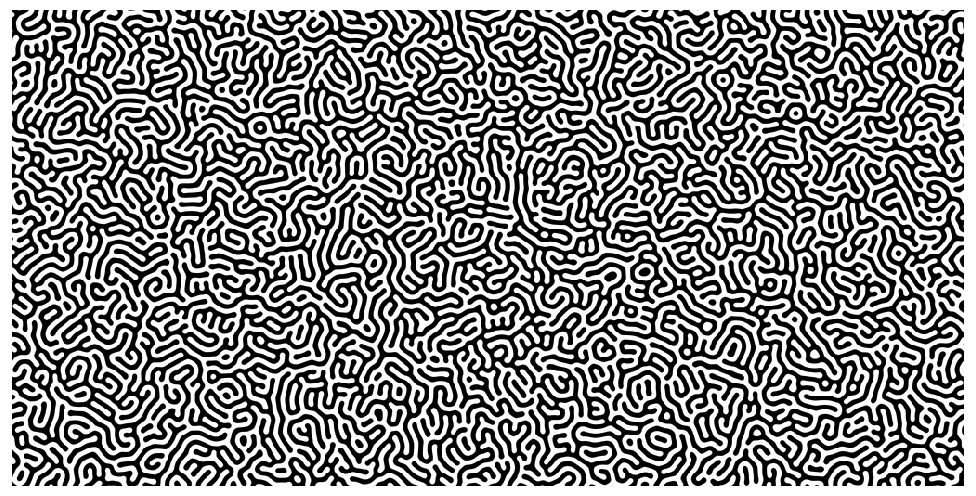
\includegraphics[angle=0,width=0.5\textwidth]{phi_run703_320.jpg}\\
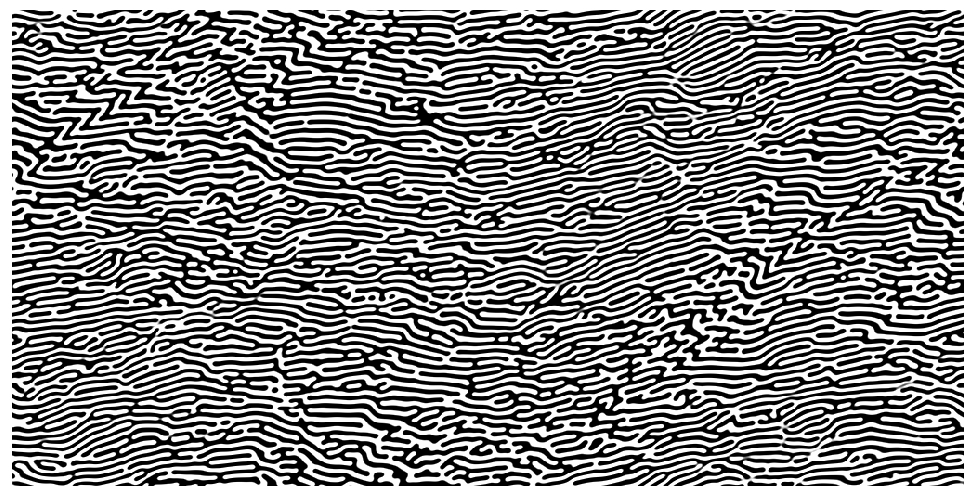
\includegraphics[angle=0,width=0.5\textwidth]{phi_run704_500.jpg}\\
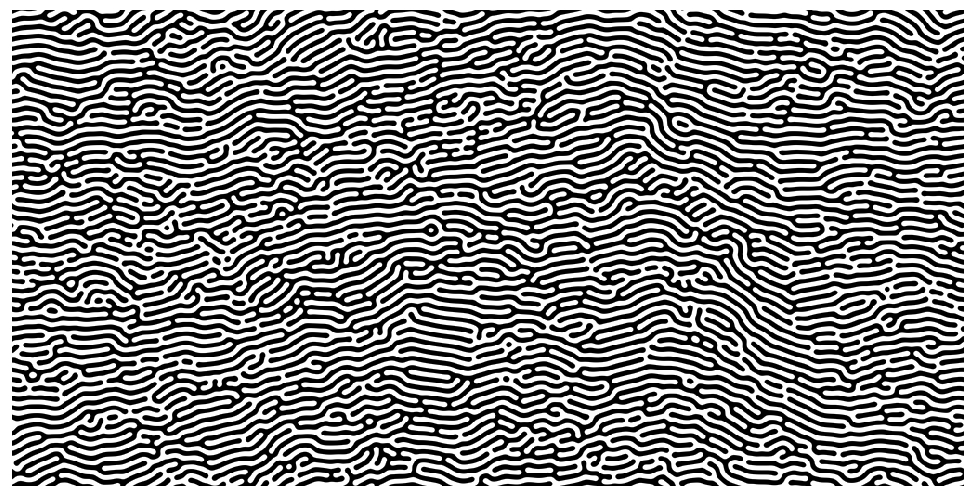
\includegraphics[angle=0,width=0.5\textwidth]{phi_run705_1280.jpg}
\caption{Order parameter $\phi$ of system A-2D: after equilibration (timestep $t=3.2\e{5}$, top), at $\dot{\gamma}=1\cdot10^{-4}$ ($t=5\e{5}$, centre) and after switch-off ($t=1.28\e{6}$, bottom). Gray scaling from black to white corresponds to values of $-1\le\phi\le1$}
\label{fig1}
\end{figure}


\begin{figure}[htp]
\centering
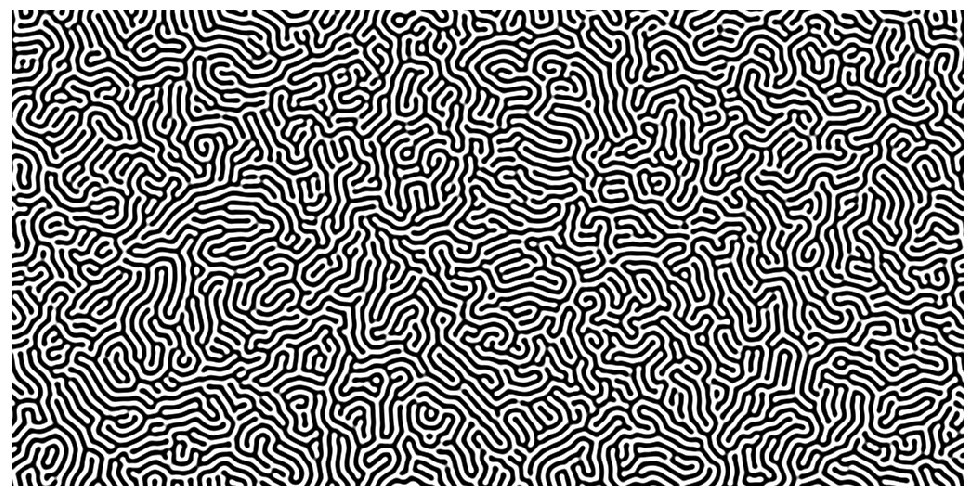
\includegraphics[angle=0,width=0.5\textwidth]{phi_run707_320.jpg}\\
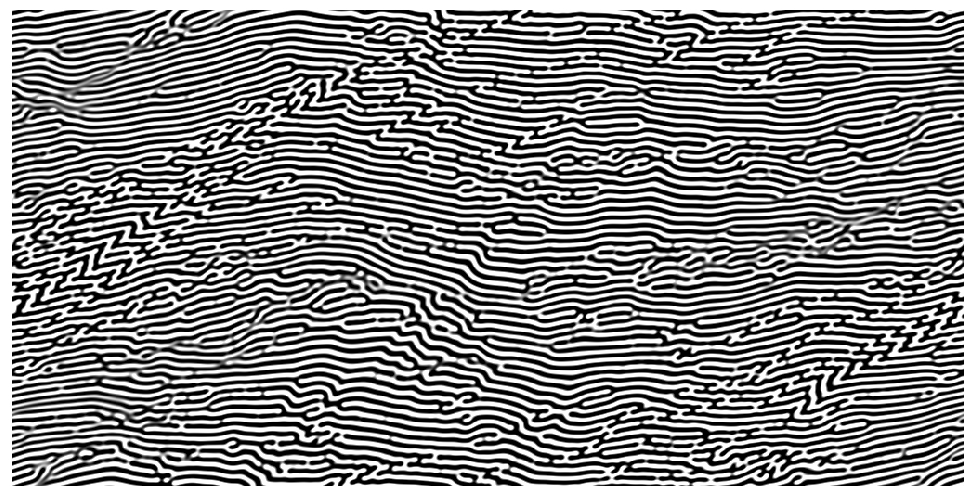
\includegraphics[angle=0,width=0.5\textwidth]{phi_run710_800.jpg}\\
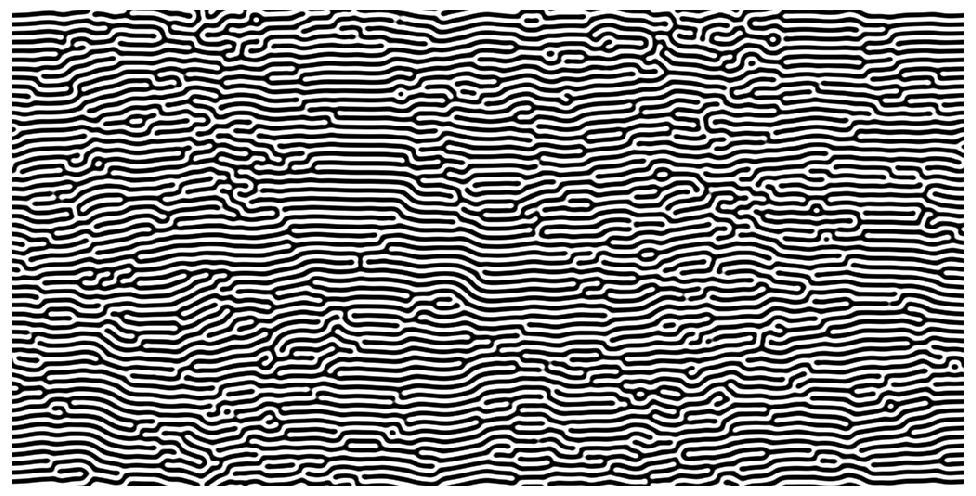
\includegraphics[angle=0,width=0.5\textwidth]{phi_run765_1280.jpg}
\caption{Order parameter $\phi$ of system B: after equilibration (timestep $t=3.2\e{5}$, top), at $\dot{\gamma}=1\cdot10^{-4}$ ($t=8\e{5}$, centre) and after switch-off ($t=1.28\e{6}$, bottom)}
\label{fig2}
\end{figure}

The flow direction and the direction of the velocity gradient are {\it vertical} x- and {\it horizontal} y-direction.
The relative flow imposed by the Lees-Edwards planes is always in positive y-direction in the upper half and in negative y-direction in the lower half of the images.
After a short transient phase during which the order parameter remains rather homogenous, regions of reduced and increased lamellar width emerge and the spacing begins to deviate from its well-defined equilibrium value.
These regions are advected with the flow while they continuously undergo affine transformations.
The centre picture in Fig. \ref{fig1} shows an example at an intermediate time step at shear rate $\gd= 1\e{-4}$.
In a previous work on binary fluids and lamellar systems in shear flow \cite{Xu06b} another shear-induced structure was found.
However, the reported results differ from our observations in the following aspects.
Xu et al. shear-induced structures emerge at the centre and remain localised, while ours do occur in band-like patterns that are wrapped around the periodic boundaries of our system.
Xu et al. also reported a shear banding region with reduced local shear rate, which is absent in our case.
These differences may be simply a direct consequence of the different boundary conditions that were applied.
While we applied Lees-Edwards BCs to all quantities, Xu and co-workers seem to have used a kind of hybrid scheme.

\begin{figure}[htp!]
\centering
\hspace*{-0.1cm}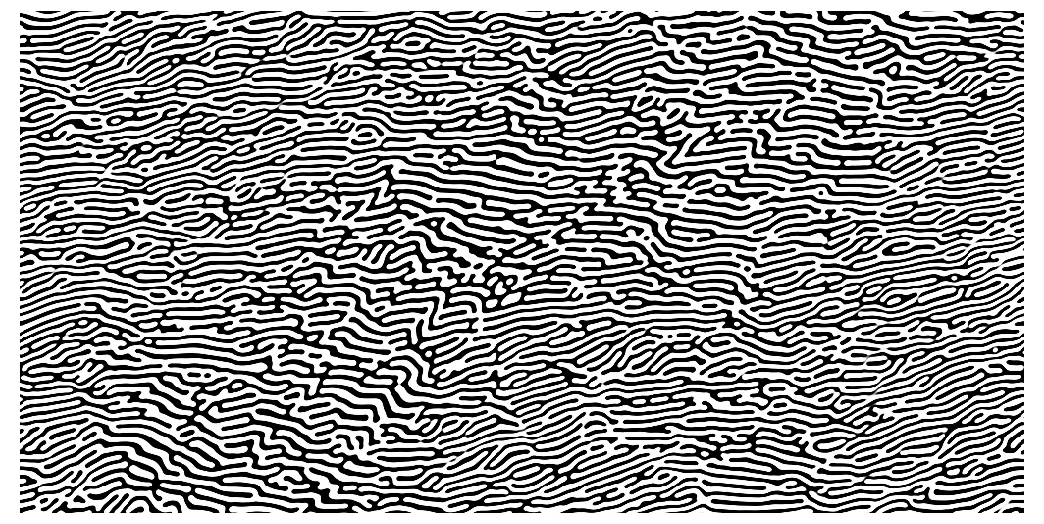
\includegraphics[angle=0,width=0.5\textwidth]{phi_run704_400.jpg}
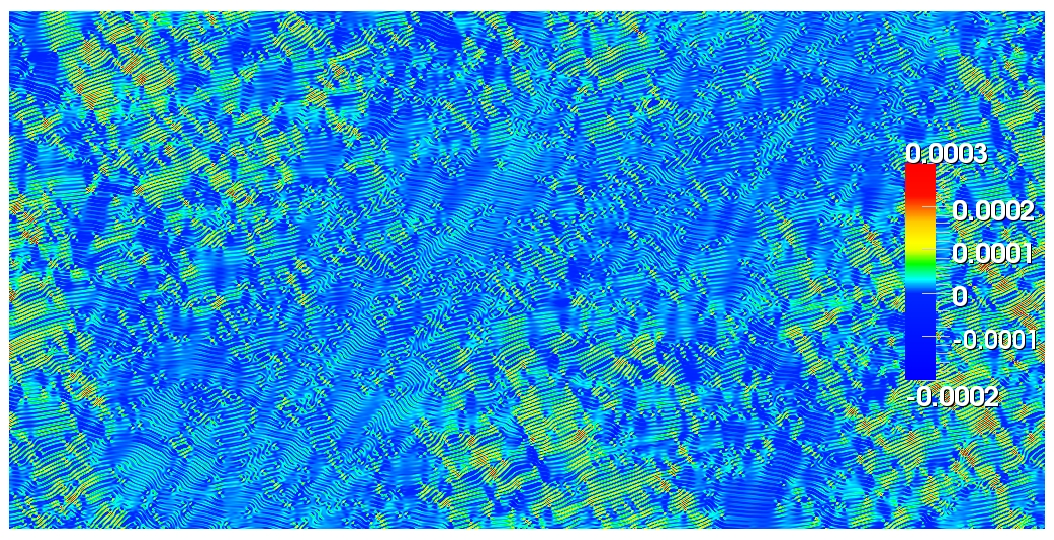
\includegraphics[angle=0,width=0.49\textwidth]{shear_str_run704_400.jpg}
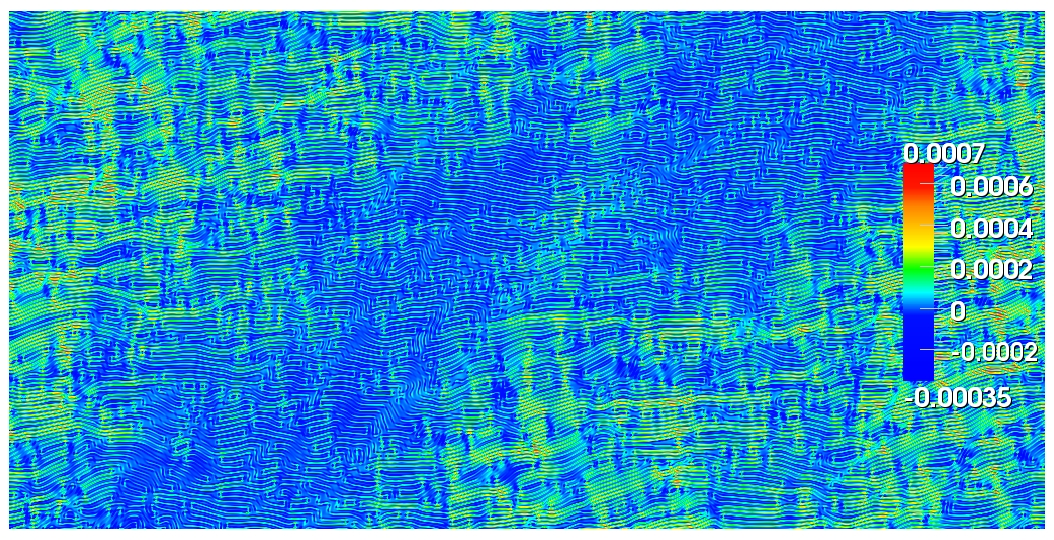
\includegraphics[angle=0,width=0.49\textwidth]{N1_run704_400.jpg}
\caption{Order parameter $\phi({\mathbf r})$ (top), shear stress $\sigma_{xy}({\mathbf r})$ (centre) and first normal stress differences $N_1({\mathbf r})$ (bottom) of system A-2D at $t=4\e{5}$}
\label{fig3}
\end{figure}

\begin{figure}[htp!]
\centering
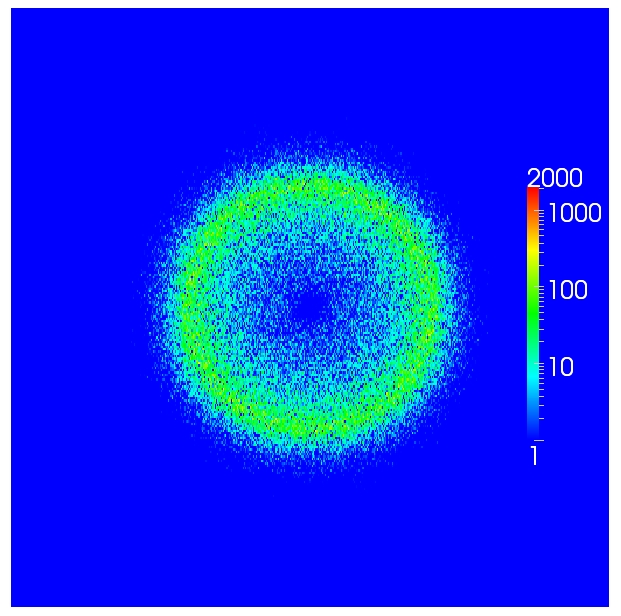
\includegraphics[angle=0,width=0.33\textwidth]{ck_run703_320.jpg}
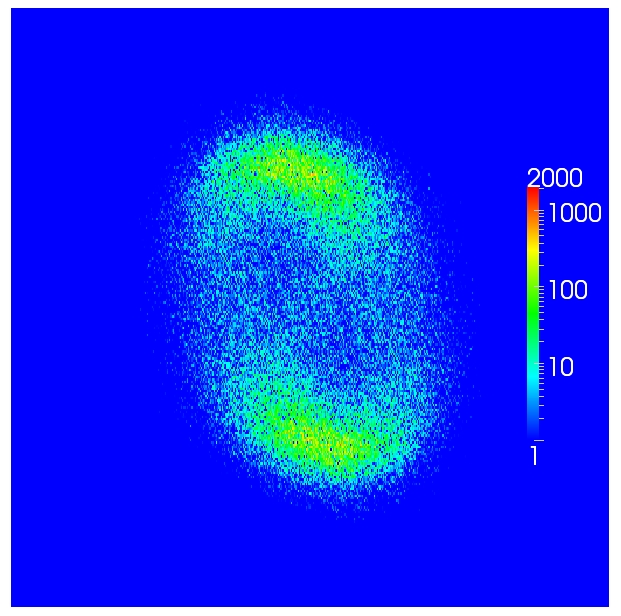
\includegraphics[angle=0,width=0.33\textwidth]{ck_run704_500.jpg}
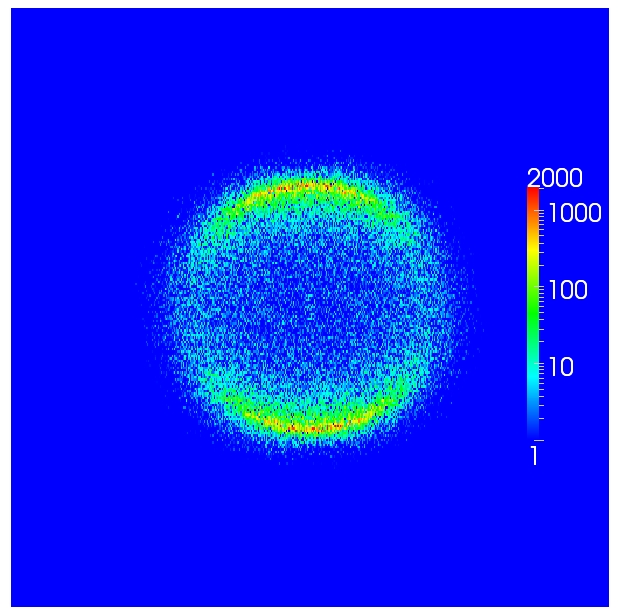
\includegraphics[angle=0,width=0.33\textwidth]{ck_run705_1280.jpg}
\caption{Structure factor $C({\bm k})$ of system A-2D: Shown are states after equilibration at $t=3.2\e{5}$ (left), at $\dot{\gamma}=1\cdot10^{-4}$ and $t=5\e{5}$ (centre) and after switch-off at $t=1.28\e{6}$ (right). The sections shown correspond to wave vectors on the interval $k_x, k_y \in [-\pi/2 l,\pi/2 l]$.}
\label{fig4}
\end{figure}

To our understanding Lees-Edwards BC were applied to the order parameter only, whereas solid moving walls were placed in the LB-part at the upper and lower boundaries.
It might be that in \cite{Xu06b} actually not bulk flow behaviour was simulated, but rather flow in a confined geometry. 
This could also explain why Xu et al. always observe a shear-induced structure at the centre of the system.\\ 
After the shear flow has been switched off the lamellar spacing became again more homogenous and the equilibrium value was restored with expanded regions contracting and vice versa.
The final state after the relaxation has virtually come to a standstill is shown in the bottom picture of Fig. \ref{fig1}. 
Most of the lamellae remain oriented along the flow direction, but depending on the local expansion and compression level during flow some regions may have large angles after relaxation. 
The length of the interfaces varies considerably, which is another residue of the inhomogeneities present in shear flow.\\
Fig. \ref{fig2} shows equivalent states for system B-2D with lower segregation.
All generic results of Fig. \ref{fig1} are the same, but the interfaces appear to be slightly longer.
Consequently, the lamellar alignment in flow direction after switch off is also more pronounced.\\ 
In Fig. \ref{fig3} we suggest a relation between the inhomogeneous morphology in the flowing state and typical rheological quantities.
The pictures show the order parameter $\phi({\bm r})$, shear stress density $\sigma_{xy}({\bm r})$ and first normal stress difference density $N1({\bm r})=\sigma_{yy}({\bm r})-\sigma_{xx}({\bm r})$ of system A-2D in steady shear flow at shear rate $\dot{\gamma}=1\e{-4}$.
In regions where the lamellar width is larger than in the equilibrium state shear stresses and first normal stress differences show low positive or negative values.
Large positive values of both quantities coincide with regions where the lamellae are under compression.
Peak values in LBU are in the region of $-2\e{-4}$ and $3\e{-4}$ for shear stress and  $-3.5\e{-4}$ and $7\e{-4}$ for the normal stress differences.
Despite being locall negative, the ensemble averages of these quantities are always positive.
Very similar results with smaller peak magnitudes are obtained for system B-2D.
Fig. \ref{fig4} shows structure factors $C({\bm k})$ for the same states as Fig. \ref{fig1}.
Initially isotropic after spinodal decomposition and equilibration, $C({\bm k})$ has a distinct peak at $|{\bm k}|\simeq \pm0.2\pi/l$.
In steady shear flow the structure factor develops two distinct but rather broad peaks at $k_x\simeq\mp 0.012\pi/l, k_y\simeq\pm 0.22 \pi/l$.
It is interesting to see that the inhomogenous morphology of the lamellar structure is also clearly encoded in the structure factor. 
The Fourier-vector at the peak has a small component in x-direction, indicating the average tilt of the lamellae away from the flow direction in the direction of extensional flow.
The position of the peak is almost constant throughout the entire simulation and the average lamellar spacing decreases from about 10 lattice sites in equilibrium to about 8.5 lattice sites.
If the shear flow is switched off the system adopts again its equilibrium value and the small tilt of the signal vanishes completely, indicating that this is a purely dynamical phenomenon. 
The intensity of the peak is slightly larger due to the fact that the interfaces remain oriented along the flow direction.
By introducing the alignment factor $X_i$ in Eq. \ref{alignment} we suggest a method to identify and quantify defects in the lamellar structure.
Fig. \ref{fig5} shows an example of the time evolution of system A-2D at low shear rate.
All lattice sites with $X_i\le0.8$ are marked in red and they obviously coincide with lamellar endpoints or local disturbances.
The top picture gives the situation at the lowest applied shear rate $\dot{\gamma}=1.25\e{-5}$, whereas the system has been pre-sheared at consecutively decreasing shear rates between $\gd=1\e{-4}$ and $2.5\e{-5}$.
There are regions which show some sort of flow alignment and others which don't.
The bottom picture of Fig. \ref{fig5} shows a later state with a total strain that has increased by another $10^{5}\%$. 
Obviously many defects have annealed and the interfaces are well aligned with the flow direction.

\begin{figure}[htp!]
\centering
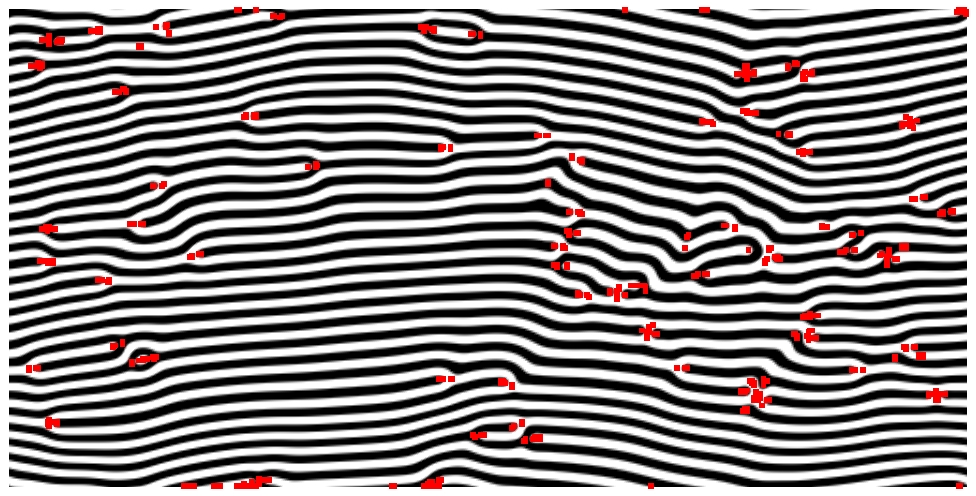
\includegraphics[angle=0,width=0.5\textwidth]{phi_defects_run774_5120.jpg}
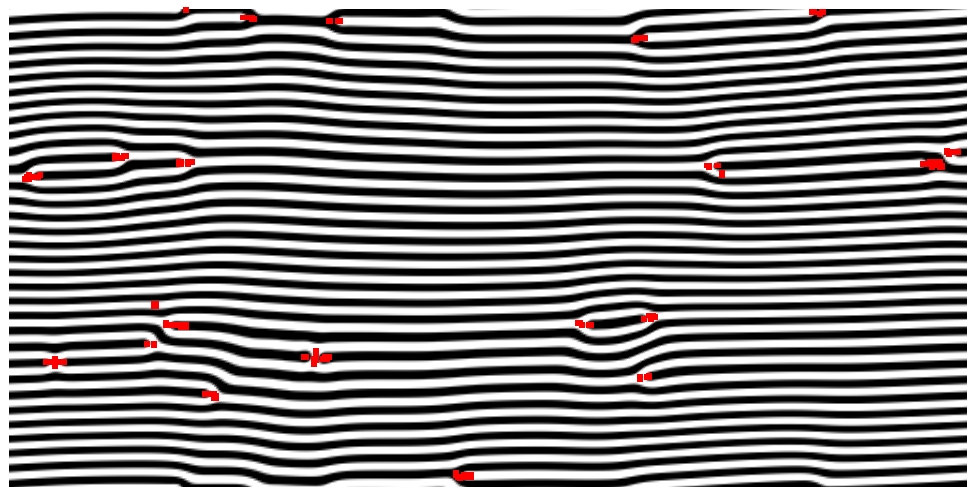
\includegraphics[angle=0,width=0.5\textwidth]{phi_defects_run774_10240.jpg}
\caption{Defect structure of system A-2D: The pictures show results at timestep $t=5.12\e{6}$ (top) and $1.024\e{7}$ (bottom) with an imposed shear rate $\dot{\gamma}=1.25\cdot10^{-5}$. The system has been pre-sheared at various higher, subsequently lowered shear rates ranging from $\dot{\gamma}=2\e{-4}$ to the above value (see Tab.\ref{tab1}). Sites where the alignment factor $X_i$ was smaller than $0.8$ are highlighted red.}
\label{fig5}
\end{figure}

Defect annihilation to this large extent is only found below a specific shear rate.
A prerequisite seems to be that the defects can smootly approach each other and cancel, which is not possible above the instability as the lamellae buckle similar to \cite{Gonnella98}, show a tendency to trip over themselves which results in the creation of new defects.
The critical value depends on the segregation and differs in systems A-2D and B-2D.
It is roughly between $\dot{\gamma}=2.5-5\e{-5}$ in A-2D and around $\dot{\gamma}=1-2\e{-4}$ in B-2D.\\
Fig. \ref{fig6} shows the  complete time evolution of the defects density $\rho_D$ of system A-2D for a sequence of decreasing shear rates starting at $\gd=2\e{-4}$ and ranging down to $\gd=2.5\e{-5}$.
The runs with the two highest shear rates were started from the equilibrium configuration, whereas all others were pre-sheared using the final configuration of the preceding run as initial configuration in order to save computational rexources.
The total strain between the beginning and end of every individual run was at least $10^{5}\%$.
Interestingly, while stepping down in shear rate both systems A-2D and B-2D anneal defects almost instantaneously.
If the shear rate is turned up again (not shown), the lamellae buckle and new defects recur immediately.

\begin{figure}[htp!]
\centering
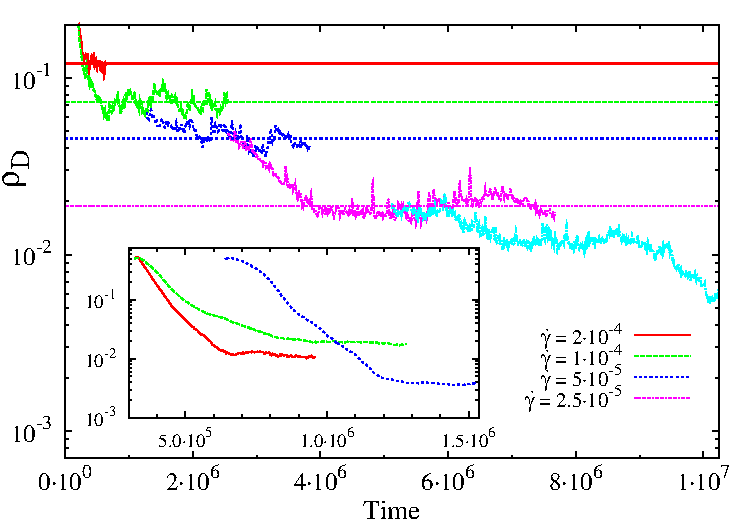
\includegraphics[angle=0,width=0.5\textwidth]{defect_density_5e-4.pdf}
\caption{Defect density $\rho_D$ vs time: The main picture shows data for system A-2D of a sequence of simulations with consecutively lowered shear rate $\dot{\gamma}=2\e{-4}$ (red solid), $1\e{-4}$ (green long-dashed),  $5\e{-5}$ (blue short-dashed),  $2.5\e{-5}$ (magenta dotted) and  $1.25\e{-5}$ (cyan dashed-dotted). Horizontal lines indicate time averages of the particular quantities, where we assume the system has reached a steady state. The inset gives data for the system A-3D and shear rates $\dot{\gamma}=2\cdot10^{-4}, 1\cdot10^{-4}$ and $5\cdot10^{-5}$.} 
\label{fig6}
\end{figure}

This finding is in further support of a dynamical equilibrium between defect creation and annihilation above a critical threshold, wheras below the critical value defects cancel and lamellae align.
To test this assumption we performed simulations starting from a very well aligned state and increased the shear rate.
The defect density goes indeed up (not shown) and reaches similar values as before.\\
Fig \ref{fig7} shows the ensemble averaged total shear stress $\langle \sigma_{xy}\rangle \equiv\sigma_{xy} $, i.e. the total shear stress per unit lattice volume.
At low shear rates stress fluctuations become actually more stretched in time and smaller, a fact that is obscured by the logarithmic scales.
In larger simulations such as those shown in Fig. \ref{fig1} and Fig. \ref{fig2} they are also about three times smaller.
Nevertheless we found that the averaged shear stress is to a very good degree independent of the system size, which makes it possible to simulate longer times using smaller system sizes without flawing the results.

\begin{figure}[htp!]
\centering
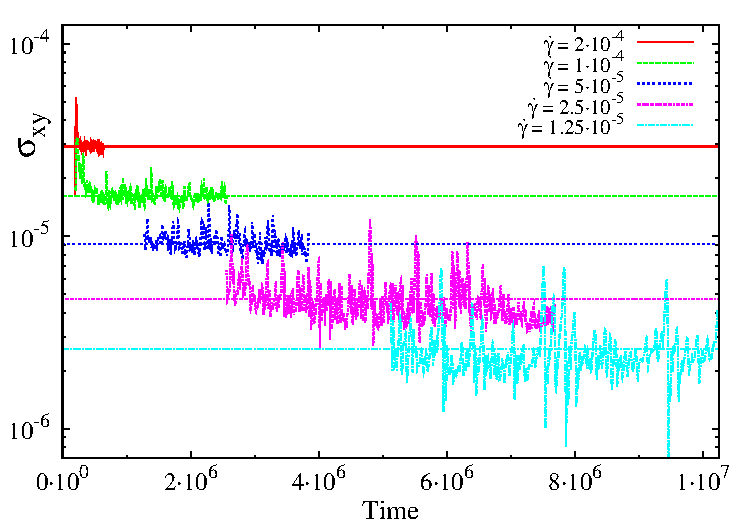
\includegraphics[angle=0,width=0.5\textwidth]{S_xy_tot_t_5e-4.pdf}
\caption{Average total shear stress $\sigma_{xy}$ versus time for system A-2D: The horizontal lines are steady state time averages. For shear rate $\dot{\gamma}=1.25\e{-5}, 2.5\e{-5}, 5\e{-5}, 1\e{-4}, 2\e{-4}$ the apparent viscosities are $\eta_{app}=\sigma_{xy}/ \eta \dot{\gamma}=2.49, 2.25, 2.18, 1.93, 1.74$.
 }
\label{fig7}
\end{figure}

System A-2D shows clear shear thinning behaviour and seems to obey a power law (see below Fig. \ref{fig11}).
Values of the apparent viscosity are given in the caption of Fig. \ref{fig7}.
Contrary to system A-2D system B-2D does not exhibit a clear tendency of shear thinning.
Here, the apparent viscosities are $\eta_{app}=1.57, 1.62, 1.55, 1.42, 1.87$ for the above shear rates and follow a more horizontal trend.\\
We want to focus now on the deviatoric part of the chemical pressure $\langle P^{chem}_{xy}\rangle\equiv P^{chem}_{xy}$.
This is shown for system A-2D in Fig. \ref{fig8}.
The fluctuations are in phase with those of the total stress in Fig. \ref{fig7} and decrease with decreasing shear rate.
In System B-2D $P^{chem}_{xy}$ decreases sharply during the run with $\gd=1\e{-4}$ (not shown) because at this shear rate pronounced defect annihilation sets in.\\

\begin{figure}[htp!]
\centering
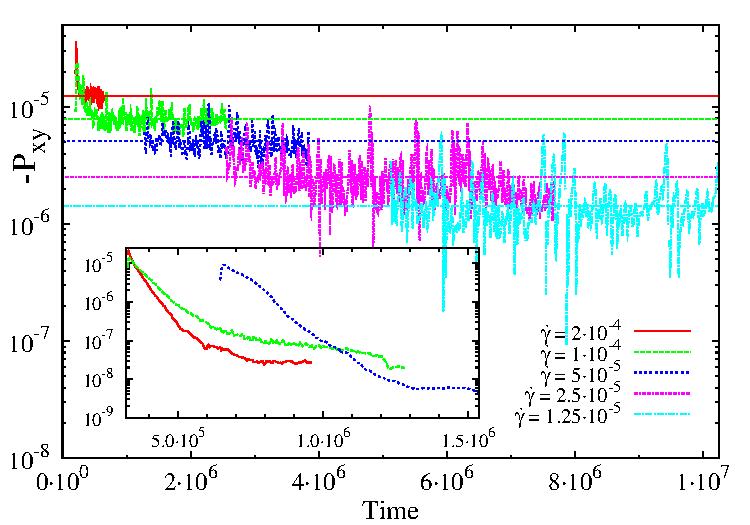
\includegraphics[angle=0,width=0.5\textwidth]{P_xy_chem_t_5e-4.pdf}
\caption{Average chemical contribution to the pressure tensor $\langle P_{xy}^{chem}\rangle$ vs time for system A-2D. The inset shows data for system A-3D and shear rates $\dot{\gamma}=2\cdot10^{-4}, 1\cdot10^{-4}$ and $5\cdot10^{-5}$.}
\label{fig8}
\end{figure}

Fig. \ref{fig9} illustrates dependence of $P_{xy}$ on the defect density $\rho_D$.
System A-2D features a linear relation between both quantities that breaks only down at the lowest defect density or rather shear rate.
The result for the softer system B-2D are less clear due to the ordering and annihilation of defects.
It is very likely that our quantifying procedure, which is based on averaging over a larger number of defects sites,is prone to inaccuracy in this regime.

\begin{figure}[htp!]
\centering
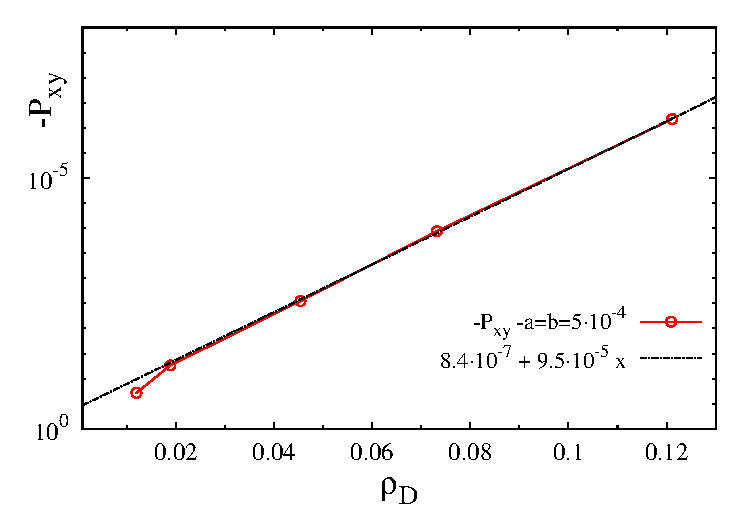
\includegraphics[angle=0,width=0.5\textwidth]{P_xy_defect_density.pdf}
\caption{Average chemical contribution to the pressure tensor $\langle P_{xy}^{chem}\rangle$ vs. defect density for system A-2D and B-2D } 
\label{fig9}
\end{figure}

Fig. \ref{fig10} shows averaged first normal stress differences $\langle N_1\rangle \equiv N_1$ versus time for system A-2D, where we followed the same protocol as before.
Initially, down till $\gd=5\e{-5}$ $N_1$ decreases monotonously with decreasing shear rate.
However, at lower shear rates the behaviour is not monotonous anymore and $N_1$ rises again.
Hence, it is difficult to define a reasonable time average for $N_1$ as for these low shear rates the system may still evolve at the end of the run.

\begin{figure}[htp!]
\centering
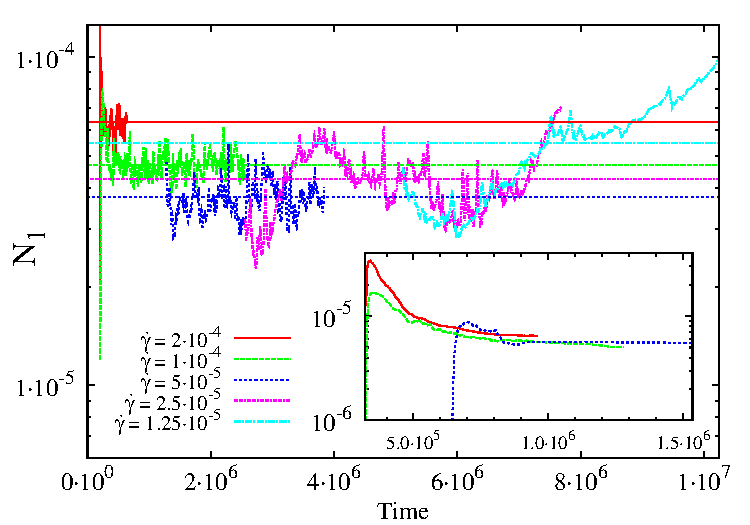
\includegraphics[angle=0,width=0.5\textwidth]{N1_t_5e-4.pdf}
\caption{Average first normal stress differences $\langle N_1 \rangle= \langle \sigma_{yy}-\sigma_{xx}\rangle$ vs time for system A-2D. The inset shows data for system A-3D and shear rates $\dot{\gamma}=2\cdot10^{-4}, 1\cdot10^{-4}$ and $5\cdot10^{-5}$.}
\label{fig10}
\end{figure}

This feature which appears somewhat erratic at first has actually a simple explanation. 
The time sequence of the defect density in Fig. \ref{fig6} reveals that the rise in $N_1$ is correlated with a drop in $\rho_D$ and linked to the defect annihilation.
When two defects meet and cancel the lamellar width increases locally by a certain amount.
This causes frustration in the system as the incommensurability between the layers is not large enough to create a new lamellar layer and allow the system to snap back towards its equilibrium width.
Hence the normal stresses $\sigma_{xx}$ become increasingly smaller and may even attain negative values, leading to gradually larger values of $N_1$.
This explanation is further sustained by the fact that only $\sigma_{xx}$ seems to evolve anomalously slowly and all other components of the stress tensor reach their steady state values more quickly.
We expect that these anomalous trends become considerably smaller in larger systems.
System B-2D behaves differently in the sense that $N_1$ does not follow this trend but rather continues to fall for lower shear rates. 
This is likely to be a direct consequence of the lower segregation in system B-2D, which gives rise to positive normal stresses $\sigma_{xx}$ preventing $N_1$ from increasing.\\
In Fig. \ref{fig11} the shear rate dependence of $\sigma_{xy}$ and $N_1$ is shown. 
System A-2D gives rise to shear thinning with the average shear stress of systems A-2D following a power law $\sigma_{xy}=\dot{\gamma}^m$ with exponent $m\simeq 0.87$.
For system B-2D the best fit is actually obtained for an exponent $m=1$, indicating more or less constant viscosity and no pronounced shear thinning.
This is because due to the decreasing number of defects at shear rates below $\dot{\gamma}\le2\e{-4}$ the chemical stress $P^{chem}_{xy}$ almost vanishes and the total stress is dominated by the hydrodynamic part.\\


\begin{figure}[htp!]
\centering
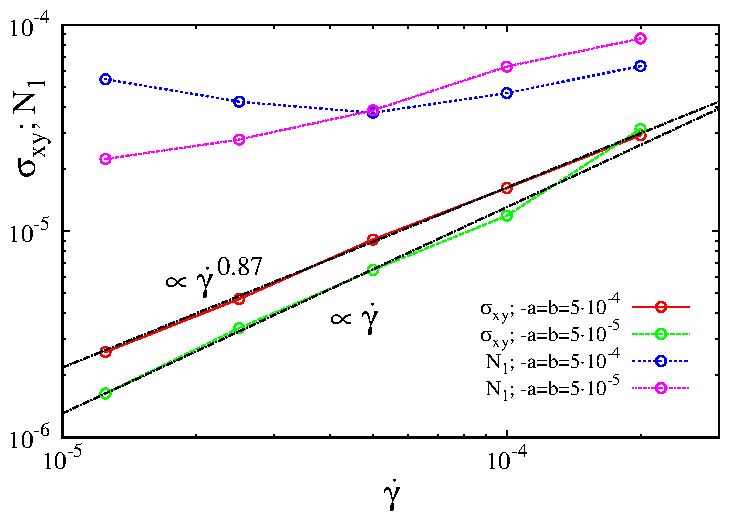
\includegraphics[angle=0,width=0.5\textwidth]{S_xy_N1_gammadot.pdf}
\caption{Flow curves: Average shear stress $\langle \sigma_{xy}\rangle$ and first normal stress differences $\langle N_1 \rangle$ vs shear rate $\dot{\gamma}$ for system A-2D ($\eta=8.33\cdot10^{-2}, -a=b=5\cdot 10^{-4}$)} 
\label{fig11}
\end{figure}

\subsection*{Results in Three Dimensions}

Because steady states require to account for large strains, the computational costs of a similar analysis of nonlinear rheology in three-dimensions are still prohibitive.
In the following we compare 3D-systems with 2D-systems smaller than those of the previous paragraph but large enough to show qualitatively similar structure under flow.

\begin{figure*}[htp!]
\centering
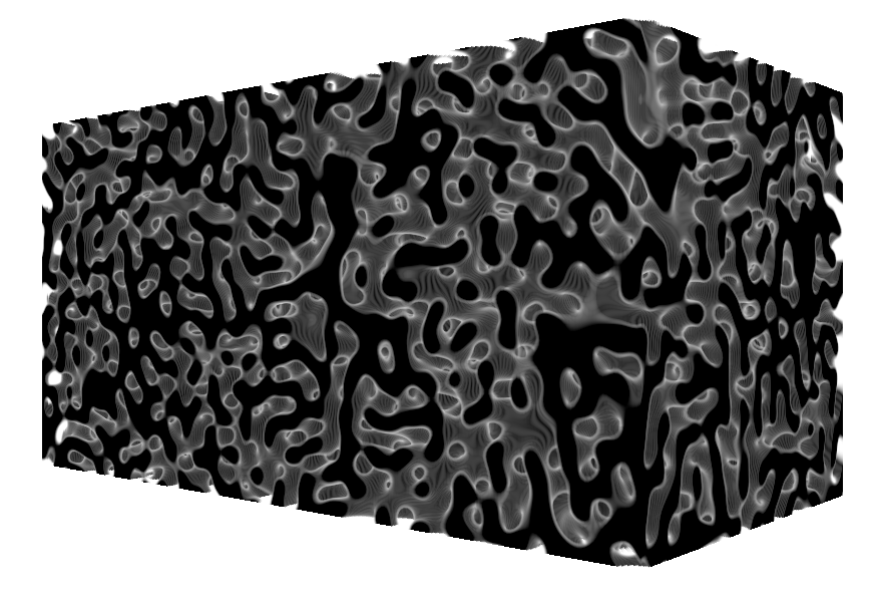
\includegraphics[angle=0,width=0.45\textwidth]{phi_run1002_320k.png}
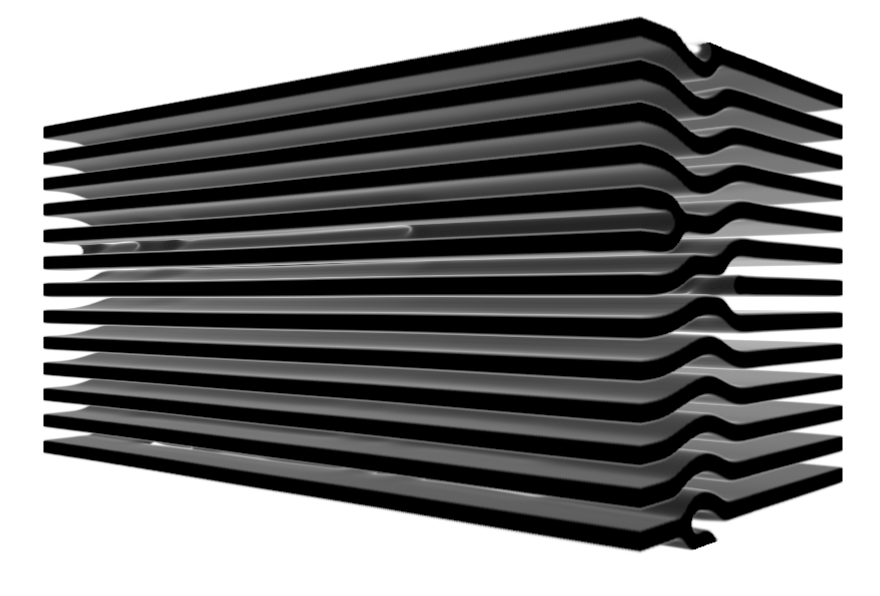
\includegraphics[angle=0,width=0.45\textwidth]{phi_run1002_640k.png}
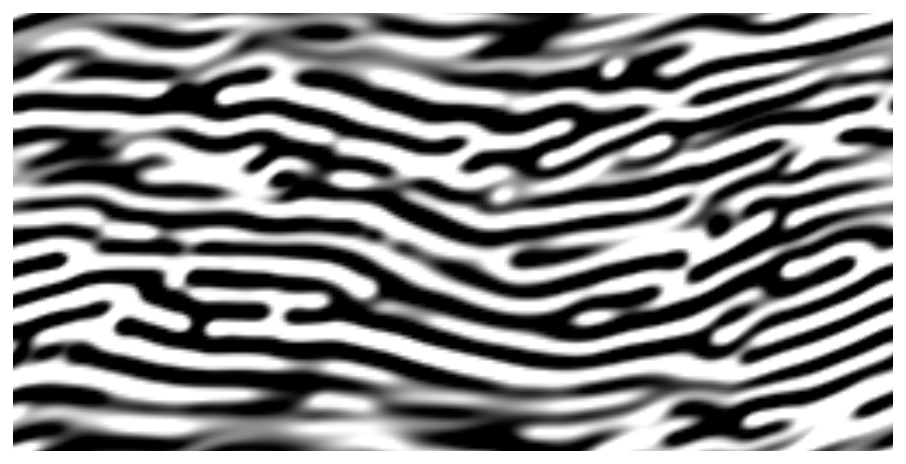
\includegraphics[angle=0,width=0.45\textwidth]{phi_run1001_640k.png}
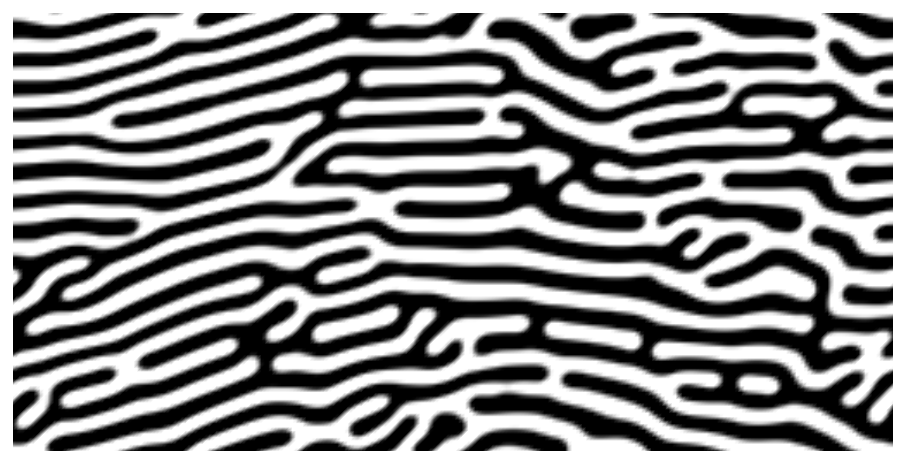
\includegraphics[angle=0,width=0.45\textwidth]{phi_run1003_960k.png}
\caption{Order parameter $\phi$ in two and three dimensions: Top pictures show system C-3D after equilibration (left) and in shear flow (right, $\dot{\gamma}=2\cdot10^{-4}$) at $t=6.4\e{5}$. The opacity of one phase has been reduced to enable a better view into the lamellar structure. The bottom left picture shows System C-2D at the same time step and shear rate. The bottom right picture is system A-2D at $\dot{\gamma}=1\cdot10^{-4}$ and time step $t=9.6\e{5}$. Results for A-3D are morphologically identical to those above.} 
\label{fig12}
\end{figure*}

The parameters sets are those of system A - we refer to A-3D for the three-dimensional run - and system C, which has a slightly larger segregation than system B.
The system size is $N_x\times N_y \times N_z=128\times256\times128$ lattice sites and $128\times256\times1$, respectively with the directions of flow along the long dimension and the velocity gradient along x in the 3D-case. 
Two snapshots of system C-2D and A-2D in shear flow are shown in the bottom pictures in Fig. \ref{fig12}.
They feature the typical fluctuating pattern of breaking and merging lamellae that was described in the previous paragraph and which is particularly pronounced in the case of system C-2D.
The top picture visualise results for system C-3D with the same free energy parameters as C-2D.
The quiescent state of system C-3D after equilibration is shown at the left with a morphology virtually identical to that of A-3D.
The lamellar width of roughly 10 lattice sites is more or less the same as in two dimensions.
A slice through the structure factor along $k_y=0$ (cuts along $k_x,k_z=0$ look identical) is shown in Fig. \ref{fig13} and resembles that in Fig. \ref{fig4}.
However, in shear flow considerable differences arise between the two- and three-dimensional case.
Contrary to the result in 2D, the three dimensional systems order readily into a regular lamellar structure after a transient period as shown in Fig. \ref{fig12} for system C-3D. 
We opted for this system as the differences between the 3D- and 2D-system are the most striking we observed.
Interestingly, these findings are consistent for even the highest shear rates, indicating that there is a very strong tendency in three dimensions to form ordered lamellar arrays.

\begin{figure}[htp!]
\centering
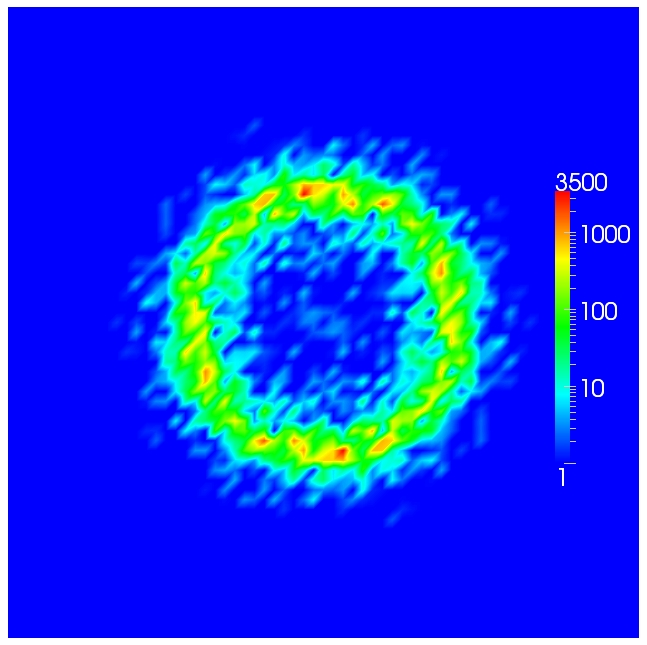
\includegraphics[angle=0,width=0.35\textwidth]{ck_y-slice_run786_320.jpg}
\caption{Structure factor $C({\mathbf k})$ of quiescent system A-3D, showing a cut along $k_y=0$ after equilibration at $t=3.2\e{5}$. Shown are wave vectors on the interval $k_x, k_z\in[-\pi/2 l,\pi/2 l]$.}
\label{fig13}
\end{figure}

\begin{figure*}[htp!]
\centering
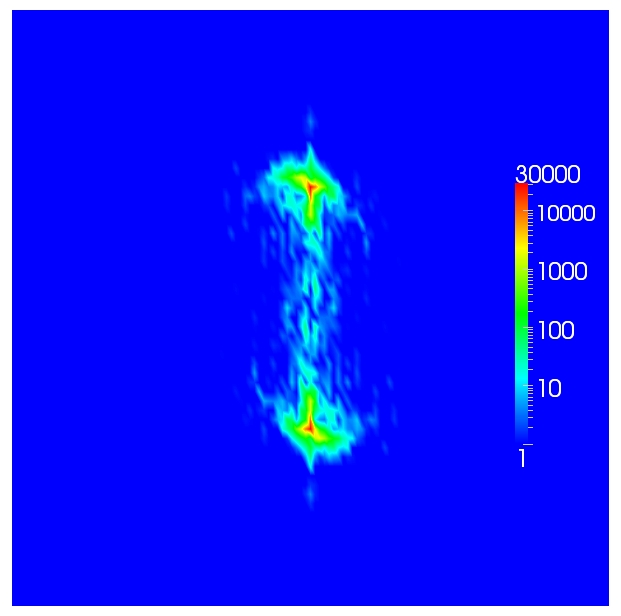
\includegraphics[angle=0,width=0.33\textwidth]{ck_x-slice_run788_960.jpg}
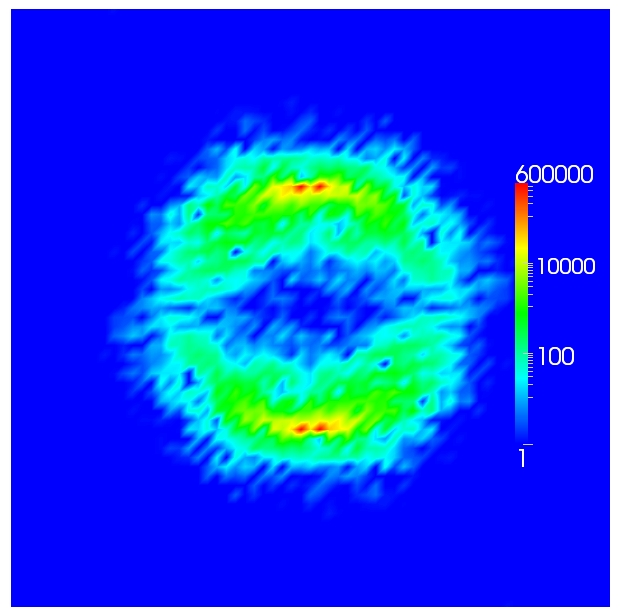
\includegraphics[angle=0,width=0.33\textwidth]{ck_y-slice_run788_960.jpg}
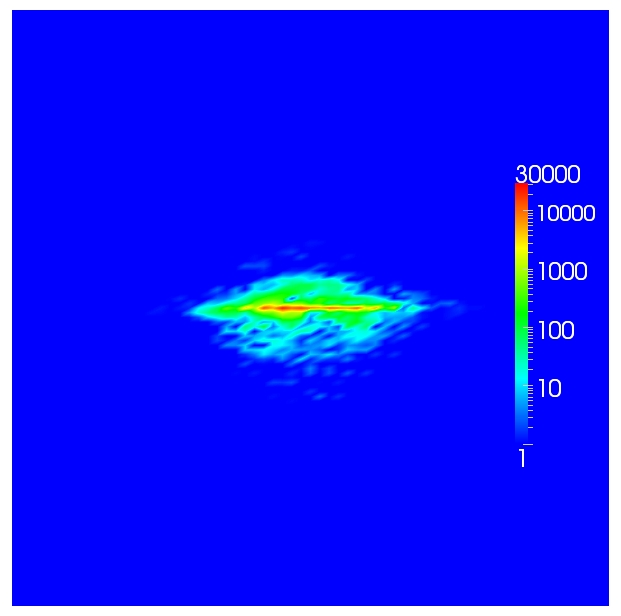
\includegraphics[angle=0,width=0.33\textwidth]{ck_z-slice_run788_960.jpg}
\caption{Structure factor $C({\mathbf k})$ of system A-3D in shear flow ($\dot{\gamma}=1\cdot10^{-4}$) at t=960k: Cuts through along $k_x=0,k_y=0$ and $k_z=3\pi/16 l$, respectively are shown for wave-vectors $k_x, k_y, k_z\in[-\pi/2 l,\pi/2 l]$. Note that in these images y is the flow direction, whereas the direction of the velocity gradient and vorticity are z and x, respectively.}
\label{fig14}
\end{figure*}

Nevertheless, the order is not completely perfect and edge dislocations emerge spontaneously in pairs as a consequence of a mismatch between some of the layers.
The Burgers vector is oriented along the gradient direction with edges along the flow direction.
This forms a structure that is translational invariant along the flow direction and in the steady state the location of the edge defects does not change and the defects to not anneal.
A closer look at the kinetic evolution of the order parameter reveals that regions separated by different values of order parameter connect along a third direction by expelling regions with opposite order parameter.
This is a direct consequence of the additional dimension and seems to play a key role during the formation of homogeneously layered structure.\\
It is instructive to quantify the time it takes system A-3D to emerge as lamellar ordered structure starting from an isotropic initial configuration.  
The inset of Fig. \ref{fig6} gives the defect density as defined by Eq. \ref{defect density} versus time for shear rates $\dot{gamma}=5\cdot10^{-5}-2\cdot10^{-4}$. 
Within a few $10^5$ timesteps the defect density decreases to magnitudes, which we obtained in case of system A-2D for shear rates about one decade lower.
The total strain where the curves level off and ordering is achieved scales with the shear rate and is about $\gamma=1.3$ ($\dot{gamma}=2\cdot10^{-4}$), $\gamma=0.8$ ($\dot{gamma}=1\cdot10^{-4}$) and $\gamma=0.6$ ($\dot{gamma}=5\cdot10^{-5}$).
 \\
A lower number of defects yields smaller chemical pressure, which is shown for the deviatortic part $P_{xy}$ in the inset of Fig. \ref{fig8}.
This contribution to the total stress is dwarfed by the hydrodynamic part and system A-3D exhibits shear thinning almost to an ultimate degree.
A relation between the magnitude of the deviatoric part of the chemical pressure and the defect density like that in Fig. \ref{fig9} in the two-dimensional case cannot be deduced.\\
First normal stress differences $N_1=\langle\sigma_{yy}-\sigma{zz}\rangle$ for system A-3D are shown in the inset of Fig.\ref{fig10}.
For all shear rates $\gd5\e{-5}-2\e{-4}$ system A-3D takes similar values, which are monotonously approached and about one decade smaller than those of system A-2D.\\ 
Finally we want to glimpse at the structure factor of system A-3D in shear flow.
Fig. \ref{fig14} shows $C({\bm k})$ at shear rate $\gd=1\e{-4}$ for Fourier vectors on the interval $[-\pi/2 l, \pi/ 2 l]$.
The leftmost picture is a cut along $k_x=0$ in with $k_y$ in horizontal and $k_z$ in vertical direction.
It shows data in flow-velocity-gradient plane and can be directly compared with the left picture in Fig. \ref{fig4}.
The other images give cuts along $k_y=0$ in $k_x-k_z$-plane and along $k_z$ in $k_x-k_y$-plane. 
Note that for the centre picture a logarithmic colour map had to be adopted due to the strong ordering in 3D.
There is a certain similarity between the 2D-structure factor {\it after} switch-off (Fig. \ref{fig4}) and the 3D-structure, but the latter shows a pronounced peak at $k_z\simeq\pm0.2\pi/l$ also during shear flow, which is slightly concealed by the logarithmic scale.The split nature is an effect of the relatively sparse discretization and was caused by the visualisation software.
Although strongly peaked, the spatial dependence of the signal is best demonstrated in a 3D-representation. 
Fig. \ref{fig15} depicts a close up of the 3D-structure factor, whereas the red area corresponds to an isosurface of about $C({\bm k})\simeq 10^3$.
It reveals a banana-shaped spatial dependence with some small appendices in flow direction at $k_x=0$.

\begin{figure}[htp!]
\centering
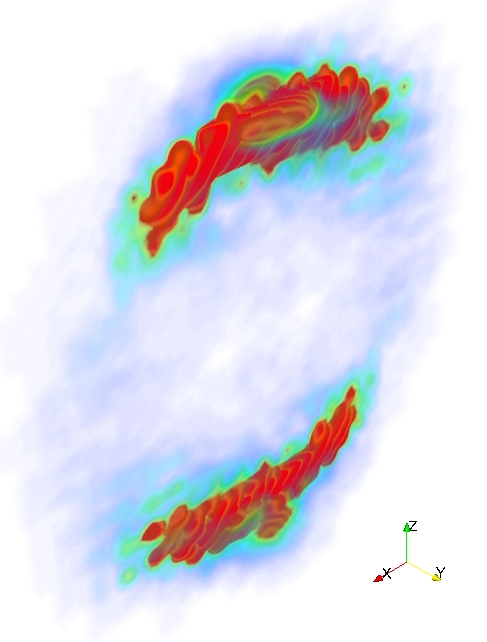
\includegraphics[angle=0,width=0.45\textwidth]{ck_run788_960_zoom.jpg}
\caption{Structure factor $C({\mathbf k})$ of system A-3D in shear flow: The picture gives a 3D-representation of the data in shear flow at $t=9.6\e{5}$ and $\dot{\gamma}=1\cdot10^{-4}$.}
\label{fig15}
\end{figure}

\section{Discussion and Conclusions}

We have performed large scale simulations of a lamellar system in steady shear flow  in two and three dimensions.
We were able to relate the morphology of the order parameter in the quiescent state to results from previous studies of the same system using similar parameters.\\
In two dimensions and steady state simple shear flow at Peclet numbers ${\cal O}(10)$ we did not observe a homogenous lamellar structure for shear rates above a critical threshold, which depends on the exact parametrization of the free energy functional.
The morphology was rather inhomogenous instead, exhibiting regions that are under pressure with lamellar spacings smaller than the equilibrium value and others that were stretched.
We could relate the structure to typical values of rheological quantities.
Areas under extensional flow coincide with locally negative or small positive shear stresses and first normal stress differences, whereas both go to positive peak values in the compressed domains.
Below a critical shear rate the systems showed no tendency anymore to trip over itself and defects annealed as they could approach each other in adjacent lamellae.
The characteristic time of this process was set by the shear rate and the total strain.
The deviatoric part of the chemical pressure was correlated to the number of defect sites, whereas the latter was measured by means of an alignment factor, which quantified the local curvature of the lamellar interfaces.
For the stiffer system A-2D we could verify a linear relation between the defect density and the average chemical contribution to the shear stress.\\ 
In system A-2D first normal stress differences decreased as long as a dynamic equilibrium between defect creation an annihilation existed.
Below the critical threshold this was no longer the case and pronounced defect annealing caused a rise in the first normal stress differences as the average lamellar spacing increased.
We could establish a shear thinning regime for the more defect laden system A-2D.
System B in contrary was so perfectly annealed in the steady state that virtually shear stresses were down at the hydrodynamic level and the relation between shear stress and shear rate was trivially linear.\\
In three dimensions we simulated shear strains which have not been attained so far.
Interestingly for the same parameters we observe striking differences between system A-2D in 2D and system A-3D in 3D.
It seems that the dynamics of the defects in two and three dimensions is rather incommensurable.
Even at the lowest applied shear rates the chemical stress has decayed to a level where the apparent viscosity was virtually identical to the solvent.
Structure factor data confirmed the very regular layered ordering of the structure and a lamellar spacing close to the equilibrium value. 

A comparison of these results with experimental work can be only limited because the topology is different in two and three dimensions.
Our 2D-systems correspond to are translational invariant along the third dimension.
Every branching point or endpoint of a lamella has the topology of an edge defect in the 3D-continuation of the structure.
A recent experimental and theoretical work studies the nonlinear relation between shear stress and shear rate in lyotropic lamellar phases \cite{Lu08}
Interestingly the authors identify the motion of screw defects as being responsible for the layer tilting, floding  and formation of defects. 
For the power law dependence of the shear stress on the shear rate Lu et al. find an experimental value of $m\simeq=1/1.44\simeq 0.694$, which is in good agreement with their theoretical prediction of $m=2/3$.
Our value of $m=0.87$ appears to be slightly too large.
A possible explanation for this is that screw defects, which do not exist in our 2D-picture, play a key role for this theory.\\



\section{Acknowledgements}
We acknowledge support by EPSRC Grants No. EP/E045316 and No. EP/E030173 and computing time at the Argonne Leadership Computing Facility, Argonne, U.S.A. as well as on HECToR, U.K.
We like to thank A. Morozov for useful discussions. 
M.E.C. holds a Royal Society Research Professorship.

\section{Appendix: Sliding Periodic Boundary Conditions}

The simulations of shear flow are undertaken using a mixed finite
difference / lattice Boltzmann approach, where the former is used
to advance the order parameter in time via the Cahn-Hilliard equation,
and the later is used to solve the Navier-Stokes equations.
Coupling between the two is
via the velocity field, which advects the order parameter, and
the thermodynamic pressure tensor (6), the divergence of which
contributes a body force on the fluid. The sliding periodic
boundary conditions of Lees and Edwards\cite{leesedwards} may be
applied to the lattice Boltzmann part of the calculation
\cite{Wagner02,Adhikari05} to generate shear in the system. We
describe here how the sliding periodic boundaries are extended to
include the finite difference part of the calculation.

We consider a finite difference mesh where the order parameter
values are co-located with the density and velocity fields provided
by lattice Boltzmann. Away from the sliding periodic boundaries, the
finite difference discretisation is as one would expect.
In order to ensure conservation of order parameter, as expressed by
\begin{equation}
\partial_t \phi + \partial_\alpha (u_\alpha \phi - M\partial_\alpha \mu) = 0,
\end{equation}
we consider each lattice point to be surrounded by a cubic control volume or
cell
of dimensions $\Delta x = 1$ in two or three dimensions.
We compute convective and diffusive fluxes at the cell boundaries using
linear interpolation of the normal velocity component to the cell face.
For the advective fluxes, the interfacial values of the order parameter
are computed via cubic interpolation weighted in the upwind direction.
This is combined with an Euler forward step for the time integration:
a small Courant number ($u\Delta t/\Delta x$), and hence numerically
stability, is guaranteed by the small Mach number constraint
standard in lattice Boltzmann. The gradient of the chemical potential
is computed at each cell face using values of $\mu$ computed at the
lattice point either side.

A body force on the fluid in the Navier-Stokes equations may be
included in the lattice Boltzmann approach. Again, to ensure conservation
of momentum, the divergence of the thermodynamic pressure tensor is
computed based on cell-face values. In practice, this requires a
finite difference stencil
that entends at least $\pm 3$ lattice points in each coordinate direction
(the thermodynamic pressure involves a fourth derivative of the order
parameter).

The sliding periodic boundaries lie (conceptually) along plane
co-incident with the cell faces. Where the finite difference stencil 
overlaps a such a plane, the relative movement between the two sides
of the plane must be accounted for when computing derivatives of the
order parameter, and hence fluxes of order parameter and momentum,
near the planes. This means interpolating values of the order parameter
on each side of the plane to positions corresponding to the lattice
locations on the other side so that the finite difference stencil
can be used normally. For this study, where there are high derivatives
of the order parameter in the free energy, it is important that this
interpolation is at least cubic. Linear interpolation of the order
parameter leads to unphysical oscillations of physical quantities
such as the shear stress related to the magnitude of the velocity jump
across the sliding boundary.
With cubic interpolation, such artefacts are absent. The non-linear
nature of this interpolation means that fluxes of both order parameter
and momentum computed at the plane do not exactly match on each side.
However, this may be corrected at each sliding boundary at each time
step, restoring global order parameter and momentum conservation.



\footnotesize{
\bibliography{smectics} %your .bib file
\bibliographystyle{rsc} %the RSC's .bst file
}

\end{document}
